\section{First-Order Logic}
	\subsection{Propositional logic}
		Une proposition logique est :
		\begin{itemize}
			\item \textbf{Déclarative :} les relations entre les variables sont décrites par des phrases
			\item \textbf{Expressive :} peut présenter des informations partielles en utilisant la disjonction
			\item \textbf{Compositionel :} Si $A$ = "il pleut" et $B$ = "j'aime la biere" alors $A \wedge B =$ "il pleut et j'aime la biere"
			\item \textbf{Manque d'expressivité} pour décrire l'environnement de manière concise (ex : ne peut pas dire "les puit provoquent des brises dans les cases adjacentes")
		\end{itemize}
		
		First-Order Logic (FOL) assume que le monde contient :
		\begin{itemize}
			\item Objects : personne, voiture, maison, \dots
			\item Relation : 
			\begin{itemize}
				\item Unary : propriété avec les objets (ex odd(x))
				\item N-ary : Relations entre les objets ()
				\item Ex : la relation de fraternité est l'ensemble $(<\text{Bob, Richard}>,<(\text{Richard,Bob})>)$
			\end{itemize}
			\item Fonctions : father\_of, successeur, \dots
		\end{itemize}
	\subsection{Syntax and semantics of FOL}
		\begin{figure}[htp]	
			\centering
			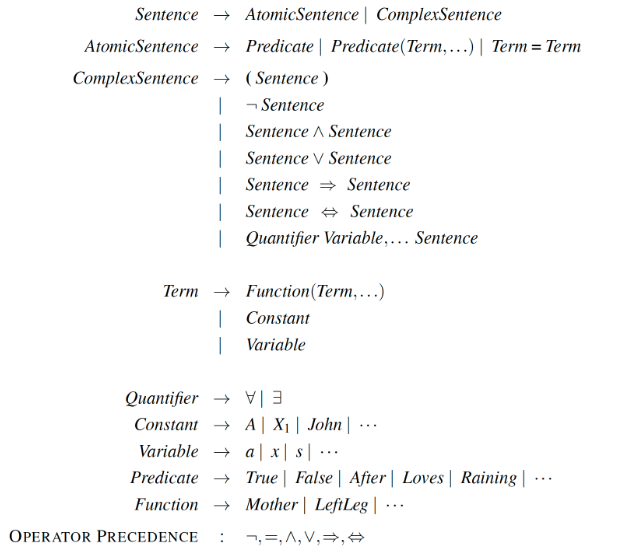
\includegraphics[width=0.6\textwidth]{img/FOL.png}
		\end{figure}
		\begin{itemize}
			\item \textbf{Alphabet :} Variables, constantes; fonctions, quantifiers, connectors \dots
			\item \textbf{Termes :} Combinaison de l'alphabet (on peut build avec les objets)
			\item \textbf{Formule bien formé} : Construite a partie de symboles de prédicats avec des termes comme arguments et à partir de connecteurs, quantifieurs et ponctuations (selon les regles des connecteurs)
		\end{itemize}
		
		\begin{figure}[htp]	
			\centering
			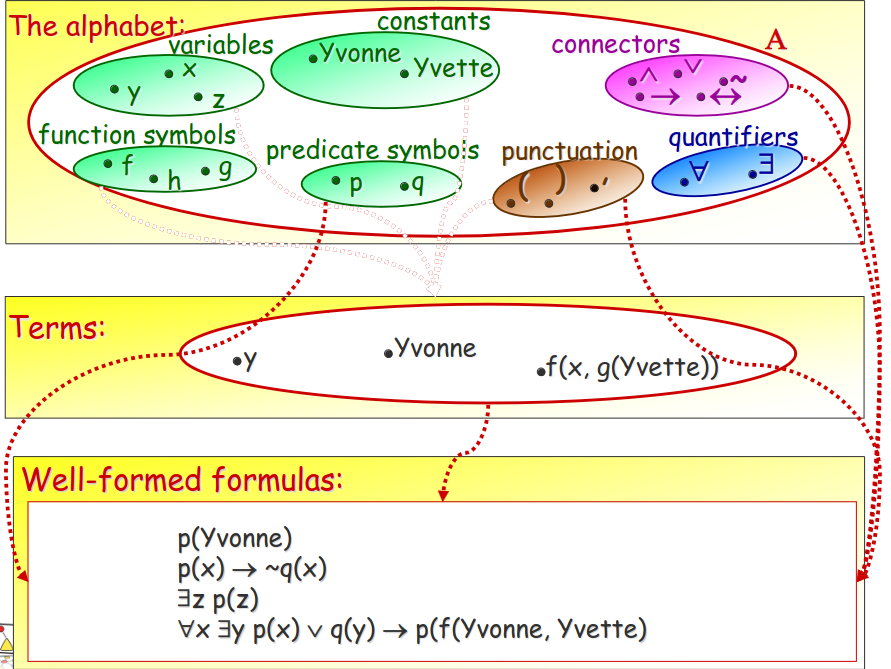
\includegraphics[width=0.6\textwidth]{img/FOL1.png}
			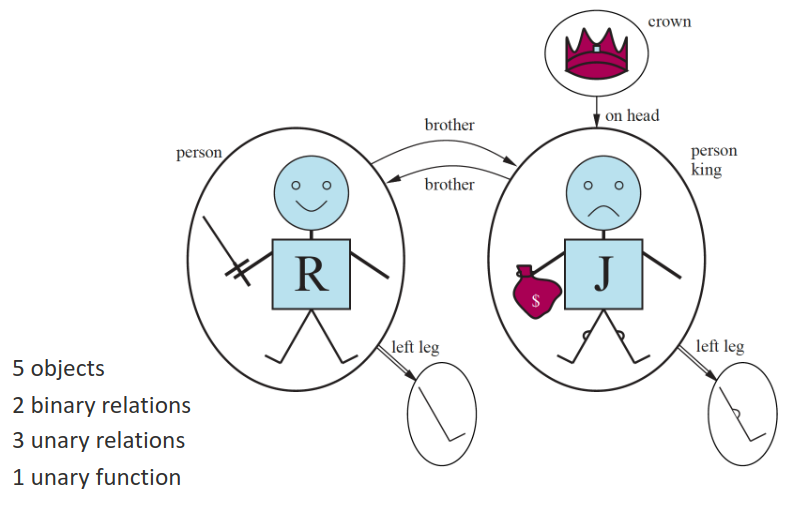
\includegraphics[width=0.6\textwidth]{img/FOL2.png}

		\end{figure}
		
		quelques exemples :
		\begin{itemize}
			\item Brother(Bob,Richard)
			\item Married(Father(Richard), Mother(Bob))
			\item King(Richard) $\land$ King(Bob)
			\item $\forall x$ King($x$) $\Rightarrow$ Person($x$)
			\item $\exists x$ Crown($x$) $\Rightarrow$ OnHead($x$)
			\item $\forall s$ Breeazy($s$) $\Leftrightarrow$ $\exists r$ Adjacent($r,s$) $\land$ Pit($r$) 
		\end{itemize}
		
		\textbf{Sémantique}
		
			c'est donnée une signification a la syntaxe
		
			Le domaine de l'interprétation est l'ensembles des objects
			
			\textbf{Constants} : L'interprétation identifies l'object dans le vrai monde.
			
			\textbf{Symbole de prédicats} : L'interprétation spécifie les relation particuliere dans le domaine.Peut etre définie implicitement ou explicitement a travers l'ensemble des tuples d'objets qui satisfait la relations
			
			
			\textbf{Fonctions de symboles} : Identifie l'object référé par un tuple d'objets.Peut etre définie implicitement ou explicitement au travers d'une table.
			
		
		\textbf{Interprétation} : 
		\begin{itemize}
			\item D le domaine
			\item Une fonction (totale) qui map les constantes a D
			\item Une fonction (totale) qui maps les fonctions de symboles as des fonctions ($D \rightarrow D$)
			\item Une fonction (totale) qui maps les symobls prédit a des prédictions ($D \rightarrow Booleans$)
		\end{itemize}
		
		Voire exemple slidesq p18 chap 8
		
		\subsubsection{Complex sentences}
			Elle sont construite en combinant des phrase atomoque en utilisant des connecteurs logique ($\neg, \land, \lor, \Rightarrow, \Leftrightarrow$) et des parentheses.
			\begin{itemize}
				\item $ \neg$ Brother(LeftLeg(Richard), Bob)
				\item Brother(Richard, Bob) $\land$ Brother(Bob, Richard)
				\item \dots
			\end{itemize}
			
		\subsubsection{Quantifiers}
			Peut etre utiliser pour exprimer des propriétés de collections d'objet
			\begin{itemize}
				\item Plus besion d'enuméré chaque objet
				\item $\forall$ dans une conjonction (quantifier universel) ex: $\forall x \ Human(x)\Rightarrow Mortal(x)$
				\item $\exists$ dans une disjonction (quantifier existentiel) ex : $\exists x \ Bird(x) \land Can\_Fly(x)$
			\end{itemize}	
			
			Attention $\forall x \forall y$ est la meme chose que $\forall y \forall x$ pareil pour $\exists$
			
			Mais $\exists x \forall y $ n'est pas la meme chose que $\forall y \exists x$  
			
			$\forall x P$ est pareil que $\neg \exists x \neg P$, pareil pour $\exists x P$ est pareil que $\neg \forall x \neg P$
			
	\subsection{Using FOL}
		\begin{figure}[htp]	
			\centering
			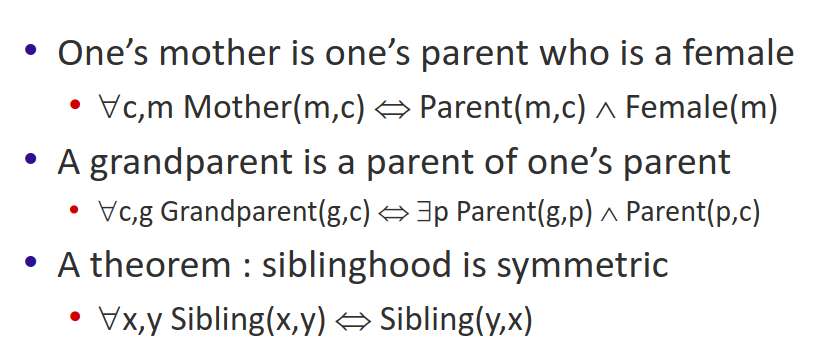
\includegraphics[width=0.6\textwidth]{img/FOL3.png}
		\end{figure}
		
		FOL peut etre utilisé pour modeliser nombre naturel, ensemble de sous ensemble, listes, ...
			
		\subsubsection{Ex Wumpus}
			\begin{figure}[htp]	
				\centering
				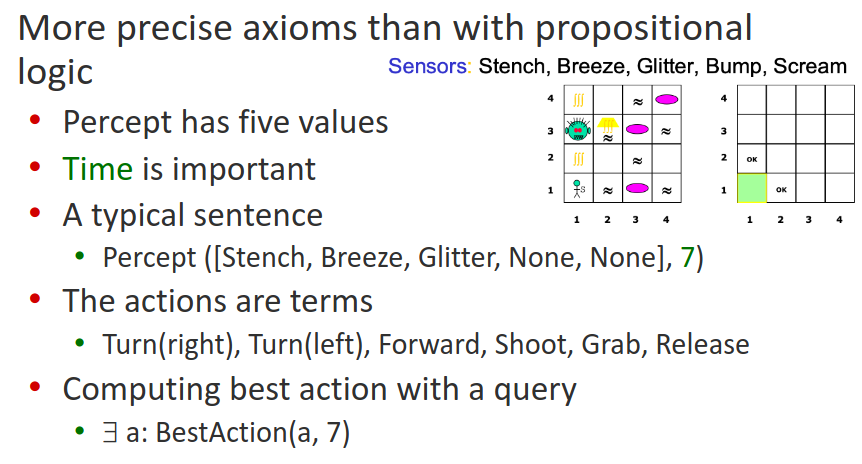
\includegraphics[width=0.7\textwidth]{img/FOL4.png}
				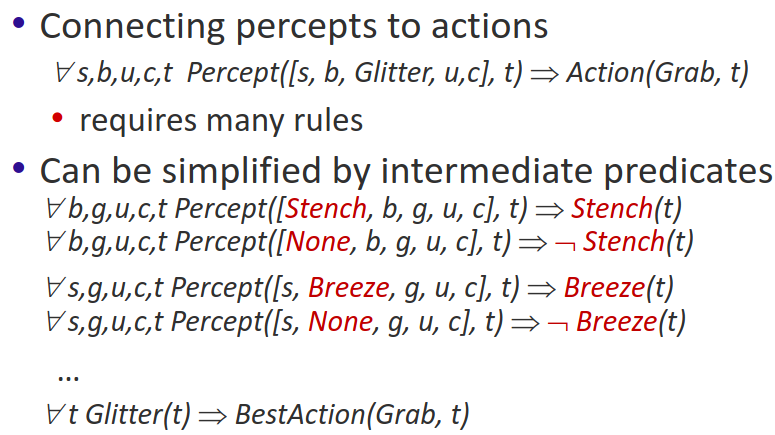
\includegraphics[width=0.7\textwidth]{img/FOL5.png}
				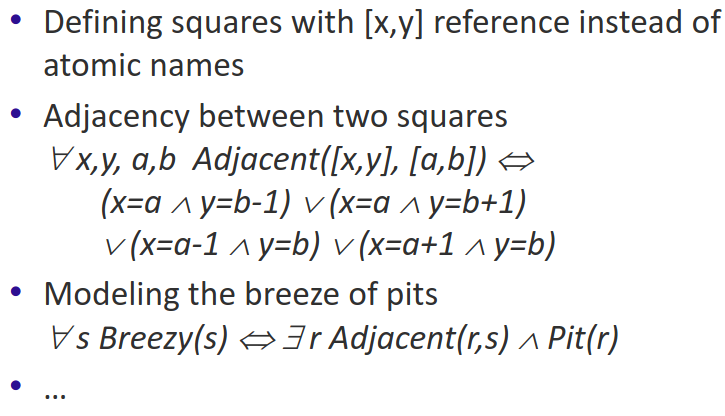
\includegraphics[width=0.7\textwidth]{img/FOL6.png}

			\end{figure}
	\subsection{Complement on FOL}
		Voir slides 41-52
		